\documentclass[conference]{IEEEtran}
\IEEEoverridecommandlockouts

\usepackage{cite}
\usepackage{amsmath,amssymb,amsfonts}
\usepackage{array}
\usepackage{graphicx}
\usepackage{textcomp}
\usepackage{xcolor}
\usepackage{url}
\usepackage[hidelinks]{hyperref}
\usepackage{tikz}
\usetikzlibrary{shapes.geometric, arrows.meta, positioning, fit, calc, backgrounds}

\def\BibTeX{{\rm B\kern-.05em{\sc i\kern-.025em b}\kern-.08em
    T\kern-.1667em\lower.7ex\hbox{E}\kern-.125emX}}

\begin{document}

\title{MaternaQA-es: A Synthetic Spanish Clinical Question--Answering Dataset for Pregnancy and Maternal Health from Curated Medical Documents}

\author{
\IEEEauthorblockN{1\textsuperscript{st} Nicolás Hoyos-Giraldo}
\IEEEauthorblockA{\textit{Facultad de Ingeniería} \\
\textit{Institución Universitaria de Envigado}\\
Envigado, Colombia \\
0009-0001-9462-1136}
\and
\IEEEauthorblockN{2\textsuperscript{nd} Jhon Hander Mejía-Muñoz}
\IEEEauthorblockA{\textit{Facultad de Ingeniería} \\
\textit{Institución Universitaria de Envigado}\\
Envigado, Colombia \\
0009-0008-7768-4072}
}

\maketitle

\begin{abstract}
Spanish clinical natural language processing has limited open question--answering resources focused on pregnancy and maternal health. We present MaternaQA-es, a synthetic Spanish clinical question--answering dataset derived from curated medical documents. Its construction pipeline extracts text from PDFs, removes noisy and non-clinical pages, builds clinically meaningful chunks, generates source-grounded question--answer pairs, assigns document-level splits, and applies post-hoc quality assessment. The release contains 5,727 question--answer pairs from 1,953 chunks and 57 PDFs. Each record preserves provenance metadata, including source document, pages, chunk, split, question type, difficulty level, and supporting context. MaternaQA-es is distributed as three JSONL views: closed-book supervised fine-tuning, grounded context-question-answer, and flat audit records. The paper reports dataset composition, topic coverage, split integrity, grounding analysis, and RAGAS-based faithfulness and answer-relevancy estimates.
\end{abstract}

\begin{IEEEkeywords}
clinical NLP, Spanish medical dataset, maternal health, pregnancy, synthetic question answering, dataset documentation, supervised fine-tuning, retrieval-augmented generation
\end{IEEEkeywords}

\section{Introduction}
Question--answering (QA) datasets have shaped progress in natural language processing by making tasks measurable, reusable, and comparable across systems. General-domain resources such as SQuAD and Natural Questions established influential dataset construction patterns for reading comprehension and open-domain QA, including clear source selection, annotation protocols, dataset analysis, and baseline evaluation \cite{Rajpurkar2016SQuAD,Kwiatkowski2019NaturalQuestions}. Biomedical QA datasets extended this paradigm to medicine, including PubMedQA for biomedical research abstracts \cite{Jin2019PubMedQA}, MedQuAD for medical consumer-health questions from trusted sources \cite{Abacha2019MedQuAD}, MedMCQA for medical exam-style reasoning \cite{Pal2022MedMCQA}, and BioASQ for biomedical semantic indexing and QA challenges \cite{Tsatsaronis2015BioASQ}. However, Spanish-language resources focused specifically on pregnancy and maternal health remain limited compared with English and broad-domain biomedical QA datasets.

Pregnancy and maternal health form a clinically important domain for language technologies. The domain includes preventive care, antenatal risk stratification, fetal monitoring, hypertensive disorders of pregnancy, diabetes in pregnancy, labor and delivery, postpartum complications, infection, medication safety, and newborn care. These topics require precise terminology, source grounding, and careful documentation. Dataset construction in this area therefore needs to report not only the final examples, but also the provenance of source material, the rationale for inclusion and exclusion, the transformation from source text to QA pairs, and the quality controls applied before release.

This paper introduces \textbf{MaternaQA-es}, a synthetic Spanish clinical QA dataset for pregnancy and maternal-health research. MaternaQA-es is a curated dataset with explicit source traceability, document-level splits, multiple publication variants, quality assessment, and release documentation. This framing follows current calls for transparent dataset documentation, including datasheets for datasets \cite{Gebru2021Datasheets}, data statements for NLP \cite{Bender2018DataStatements}, and data cards \cite{Pushkarna2022DataCards}.

The contributions of this work are fourfold:
\begin{itemize}
    \item We introduce MaternaQA-es, a synthetic Spanish clinical QA dataset focused on pregnancy and maternal health.
    \item We document a source-traceable construction methodology from curated medical PDFs, including extraction, cleaning, chunking, synthetic QA generation, and document-level split assignment.
    \item We release three complementary dataset views: a closed-book supervised fine-tuning format, a grounded context-question-answer format, and a flat JSONL audit format.
    \item We report quality and documentation evidence, including leakage controls, topic coverage, grounding analysis, RAGAS-based faithfulness and answer-relevancy estimates, and release limitations.
\end{itemize}

This paper focuses on the dataset: its motivation, construction, documentation, quality assessment, and release package.

\section{Related Work}
\subsection{QA Datasets and Biomedical QA}
SQuAD demonstrated that large-scale QA datasets can be built by pairing source passages with crowd-authored questions and extractive answers, while also analyzing question types and model performance \cite{Rajpurkar2016SQuAD}. Natural Questions shifted the emphasis toward naturally occurring user questions and explicit annotation-quality analysis \cite{Kwiatkowski2019NaturalQuestions}. These works are relevant to MaternaQA-es not because they share the same domain, but because they establish that QA dataset papers should document collection, format, quality, and evaluation methodology.

Biomedical QA resources adapt QA design to medical information needs. PubMedQA uses PubMed abstracts to answer biomedical research questions and includes expert-labeled, unlabeled, and artificially generated subsets \cite{Jin2019PubMedQA}. MedQuAD collects medical QA pairs from National Institutes of Health sources \cite{Abacha2019MedQuAD}. MedMCQA provides a large multiple-choice medical QA benchmark covering multiple medical subjects \cite{Pal2022MedMCQA}. BioASQ organizes biomedical semantic indexing and QA challenges and emphasizes the retrieval and synthesis of biomedical evidence \cite{Tsatsaronis2015BioASQ}. More recent clinical QA work, such as RealMedQA, investigates realistic biomedical questions generated from clinical recommendations and compares human and LLM-assisted generation under verification workflows \cite{Kell2025RealMedQA}. MaternaQA-es differs from these resources by focusing on Spanish maternal-health documents and by releasing both closed-book and grounded variants from a source-traceable synthetic generation process. Table~\ref{tab:related_datasets} summarizes key characteristics.

\begin{table*}[t]
\caption{How MaternaQA-es Compares with Established QA Datasets}
\label{tab:related_datasets}
\centering
\scriptsize
\setlength{\tabcolsep}{3pt}
\begin{tabular}{|p{0.15\textwidth}|p{0.10\textwidth}|p{0.18\textwidth}|p{0.10\textwidth}|p{0.17\textwidth}|p{0.14\textwidth}|}
\hline
\textbf{Dataset} & \textbf{Language} & \textbf{Domain} & \textbf{Question--answer pairs} & \textbf{Question--answer format} & \textbf{Human-authored answers} \\
\hline
SQuAD v1.1    & English & General Wikipedia passages & 98k+ & Extractive reading comprehension & Yes \\
Natural Questions & English & General Google queries and Wikipedia pages & 300k+ & Long-form and short-answer QA & Yes \\
PubMedQA      & English & Biomedical literature abstracts & 211k  & Yes/no/maybe biomedical QA & Yes \\
MedQuAD       & English & Consumer health information & 47k   & Medical question--answer pairs & No$^*$ \\
MedMCQA       & English & Medical examinations & 194k  & Multiple-choice medical QA & No \\
BioASQ        & English & Biomedical literature & 4k+   & Multi-format biomedical QA & Yes \\
RealMedQA     & English & Clinical recommendations & 700   & Long-form biomedical QA & Yes \\
\textbf{MaternaQA-es} & \textbf{Spanish} & \textbf{Pregnancy and maternal health} & \textbf{5,727} & \textbf{Six Spanish clinical QA types} & \textbf{No} \\
\hline
\end{tabular}

\vspace{4pt}
\footnotesize $^*$MedQuAD sources answers from NIH portals; QA pairs are not individually expert-verified.

\end{table*}

\subsection{Synthetic Instruction and QA Data}
Synthetic instruction generation has become a common strategy for creating task-specific instruction-following data. Self-Instruct introduced a bootstrapping procedure for generating instruction data from language models \cite{Wang2023SelfInstruct}, and Alpaca popularized instruction tuning with synthetic examples derived from Self-Instruct-style prompting \cite{Taori2023Alpaca}. WizardLM and Evol-Instruct further explored methods for increasing instruction diversity and complexity \cite{Xu2023WizardLM}. LIMA argued that carefully curated examples can produce strong alignment behavior even at relatively small scale \cite{Zhou2023LIMA}. These works support the methodological premise that synthetic instruction-like QA examples can be useful when generation is constrained, documented, and evaluated.

MaternaQA-es applies this premise. The dataset uses LLMs to generate QA formulations, but the factual basis is the curated medical source text. The synthetic step transforms source-grounded clinical text into question--answer examples; it does not synthesize new clinical facts. This distinction is central to the dataset documentation.

\subsection{Dataset Documentation Frameworks}
Dataset papers increasingly need to describe the context and limitations of data creation. Datasheets for Datasets propose documenting motivation, composition, collection process, preprocessing, uses, distribution, and maintenance \cite{Gebru2021Datasheets}. Data Statements for NLP adapt this transparency goal to language datasets by emphasizing curation rationale, language varieties, source data, annotator demographics, text characteristics, preprocessing, ethical review, and limitations \cite{Bender2018DataStatements}. Data Cards propose concise, stakeholder-oriented documentation for dataset origins, intent, ethical considerations, and evolution \cite{Pushkarna2022DataCards}. MaternaQA-es uses these frameworks as design guidance for documenting source provenance, Spanish-language scope, preprocessing decisions, intended uses, release constraints, and maintenance needs.

\subsection{Grounded QA, Evaluation, and Downstream Adaptation}
Grounded QA is important in clinical contexts because answers should be conditioned on evidence rather than only on parametric memory. Retrieval-augmented generation (RAG) explicitly combines retrieval with generation for knowledge-intensive tasks \cite{Lewis2020RAG}. RAGAS provides reference-free metrics for evaluating aspects of retrieval-augmented generation, including faithfulness and answer relevancy \cite{Es2024RAGAS}. MaternaQA-es is not itself a retrieval system, but its grounded variant and flat audit format preserve source context for evidence-conditioned QA and future RAG studies. The closed-book and grounded variants also support supervised fine-tuning experiments, including parameter-efficient methods such as LoRA and QLoRA \cite{Hu2022LoRA,Dettmers2023QLoRA}.

\section{Dataset Design Goals}
MaternaQA-es was designed around seven goals. First, the dataset should prioritize pregnancy and maternal-health content within a broader obstetrics and gynecology source collection, rather than generic medicine. Second, it should provide Spanish-language examples, addressing a language-resource gap in clinical NLP. Third, each example should preserve source traceability through document, page, chunk, and split metadata. Fourth, the dataset should support evidence-grounded QA by retaining source context. Fifth, it should provide training-ready variants for downstream supervised fine-tuning. Sixth, it should reduce train--test leakage by splitting at the document level. Seventh, it should document limitations and non-intended uses explicitly.

\begin{table}[t]
\caption{Design Goals and Implementation Choices for MaternaQA-es}
\label{tab:design_goals}
\centering
\begin{tabular}{|p{0.34\columnwidth}|p{0.55\columnwidth}|}
\hline
\textbf{Design goal} & \textbf{How the goal is implemented} \\
\hline
Maternal-health focus & Source documents and topic tags prioritize pregnancy, prenatal care, labor, delivery, postpartum care, fetal monitoring, and related risks while retaining documented adjacent topics. \\
\hline
Spanish language & Questions, answers, and source text are in Spanish. \\
\hline
Source traceability & QA records retain source PDF, page, chunk, topic, role, and split metadata. \\
\hline
Grounded use & A grounded SFT variant includes source context with the question. \\
\hline
Training readiness & Conversational JSONL variants are produced for supervised fine-tuning. \\
\hline
Leakage control & Splits are assigned at document level. \\
\hline
Release boundaries & The dataset documentation identifies limitations and non-intended uses. \\
\hline
\end{tabular}
\end{table}

\section{Source Corpus}
The source corpus consists of Spanish medical PDFs stored in the project repository under the source-document collection. The collection includes clinical practice guidelines, protocols, manuals, academic chapters, review articles, and institutional documents related to pregnancy, maternity care, obstetrics, perinatal care, and adjacent maternal-health topics. Each PDF is registered in a document inventory with technical and inclusion metadata such as file name, path, page count, document type, language, inclusion status, OCR indicators, and exclusion reasons.

Table \ref{tab:corpus_stats} summarizes the current corpus processing state. The pipeline processed 63 PDFs and extracted 5,856 pages. After cleaning and filtering, 5,176 pages were retained and 660 pages were discarded. The most common discard reason was the need for OCR, followed by pages that were too short, reference-heavy, fragmented, table-of-contents or index pages, and non-clinical sections.

\begin{table}[t]
\caption{Corpus Size After PDF Extraction, Cleaning, and Chunking}
\label{tab:corpus_stats}
\centering
\begin{tabular}{|l|r|}
\hline
\textbf{Processing metric} & \textbf{Count or value} \\
\hline
Processed PDFs & 63 \\
Extracted pages & 5,856 \\
Kept pages & 5,176 \\
Discarded pages & 660 \\
Pages needing OCR & 332 \\
Final chunks after deduplication & 2,268 \\
Average tokens per chunk & 879.03 \\
\hline
\end{tabular}
\end{table}

\begin{table}[t]
\caption{Why Pages Were Removed During Corpus Cleaning}
\label{tab:discard_reasons}
\centering
\begin{tabular}{|l|r|}
\hline
\textbf{Discard reason} & \textbf{Number of pages} \\
\hline
Needs OCR & 332 \\
Too short & 155 \\
Reference-heavy & 89 \\
Fragmented text & 56 \\
Index/table of contents & 14 \\
Non-clinical section & 14 \\
\hline
\end{tabular}
\end{table}

The inclusion strategy favors documents with extractable Spanish clinical content and sufficient maternal-health relevance. Documents or pages with unreliable extraction are flagged or excluded so that the limitations of the current release remain visible.

\section{Corpus Processing and Chunk Construction}

The construction pipeline transforms raw clinical PDFs into structured, source-traceable text units suitable for QA generation. Figure~\ref{fig:pipeline} outlines the end-to-end process.

Text extraction proceeds at the page level using PyMuPDF as the primary engine, with pdfplumber applied as a fallback for pages yielding fewer than 50 characters. Each extracted page retains its source document identifier and page index, enabling full traceability from generated QA pairs back to the originating clinical document.

Extracted pages undergo deterministic cleaning to remove structural artifacts including repeated headers and footers, page numbers, administrative labels, and reference-heavy sections. Pages are then classified and filtered according to six criteria: pages requiring OCR are flagged rather than auto-recovered; pages with fewer than 150 characters after cleaning are discarded as non-substantive; reference-heavy pages, fragmented text, navigational pages (index/table of contents), and non-clinical sections are excluded. This filtering strategy is intentionally conservative, prioritizing clinically meaningful language over aggressive content recovery. Of the 5,856 extracted pages, 5,176 (88.4\%) were retained and 660 (11.6\%) were discarded; Table~\ref{tab:discard_reasons} details the distribution of discard reasons. Each page retains audit metadata recording its inclusion status and applicable discard reason.

Retained pages are grouped into clinically coherent text units that balance answerability with generation constraints. The construction script applies configurable boundaries with a default minimum of 500 tokens, maximum of 1,200 tokens, and 80-token overlap between adjacent chunks. Candidate chunks are filtered by an accepted-token threshold and a clinical-score heuristic estimating the proportion of domain-relevant terminology. Each chunk receives a stable identifier and is annotated with source PDF, page range, document type, section type, content role, topic tags, token estimate, and clinical score.

Exact and near-duplicate detection is applied before publication. The audit identified one exact duplicate and two near duplicates among accepted chunks, including cross-PDF duplicates from shared clinical guidelines. After deduplication, 2,268 final chunks remained, of which 2,223 were assigned to the LM dataset splits (1,997 training, 115 validation, 111 test) and 45 were reserved for documentation examples. Split assignment operates at the document level: all chunks derived from the same source PDF are assigned to a single dataset split, preventing near-identical content from appearing in both training and evaluation subsets.

\begin{figure}[!t]
\centering
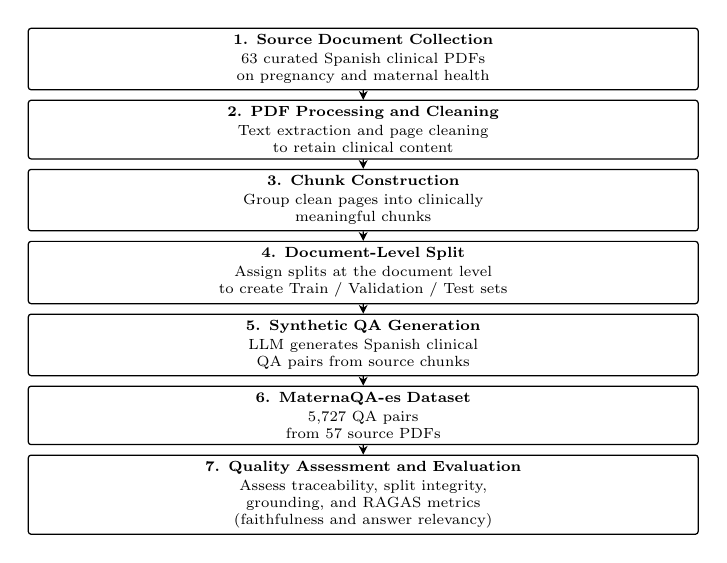
\begin{tikzpicture}[
  scale=0.76,
  transform shape,
  font=\scriptsize,
  pipelinebox/.style={
    rectangle,
    draw=black,
    line width=0.45pt,
    rounded corners=1pt,
    text width=0.90\columnwidth,
    minimum height=0.60cm,
    align=center,
    inner xsep=4pt,
    inner ysep=3pt
  },
  flowarrow/.style={
    -{Stealth[length=3.2pt,width=3.2pt]},
    line width=0.45pt,
    draw=black
  },
  node distance=0.16cm
]

\node[pipelinebox] (source) {
  \textbf{1. Source Document Collection}\\[1pt]
  63 curated Spanish clinical PDFs\\
  on pregnancy and maternal health
};

\node[pipelinebox, below=of source] (processing) {
  \textbf{2. PDF Processing and Cleaning}\\[1pt]
  Text extraction and page cleaning\\
  to retain clinical content
};

\node[pipelinebox, below=of processing] (chunks) {
  \textbf{3. Chunk Construction}\\[1pt]
  Group clean pages into clinically\\
  meaningful chunks
};

\node[pipelinebox, below=of chunks] (split) {
  \textbf{4. Document-Level Split}\\[1pt]
  Assign splits at the document level\\
  to create Train / Validation / Test sets
};

\node[pipelinebox, below=of split] (qagen) {
  \textbf{5. Synthetic QA Generation}\\[1pt]
  LLM generates Spanish clinical\\
  QA pairs from source chunks
};

\node[pipelinebox, below=of qagen] (dataset) {
  \textbf{6. MaternaQA-es Dataset}\\[1pt]
  5,727 QA pairs\\
  from 57 source PDFs
};

\node[pipelinebox, below=of dataset] (evaluation) {
  \textbf{7. Quality Assessment and Evaluation}\\[1pt]
  Assess traceability, split integrity,\\
  grounding, and RAGAS metrics\\
  (faithfulness and answer relevancy)
};

\draw[flowarrow] (source) -- (processing);
\draw[flowarrow] (processing) -- (chunks);
\draw[flowarrow] (chunks) -- (split);
\draw[flowarrow] (split) -- (qagen);
\draw[flowarrow] (qagen) -- (dataset);
\draw[flowarrow] (dataset) -- (evaluation);

\end{tikzpicture}
\caption{Overview of the MaternaQA-es construction and evaluation pipeline.}
\label{fig:pipeline}
\end{figure}


\section{Synthetic QA Generation Methodology}
The QA generation pipeline transforms curated source chunks into structured question--answer pairs using OpenAI's \texttt{gpt-5.4-mini} (May~2026 snapshot) with structured output decoding. This model was selected to balance generation quality with computational efficiency across the full corpus. The generation prompt enforces Spanish-language output with clinical precision, requiring each pair to be self-contained and grounded in the provided source context. Meta-references such as ``according to the text'' are explicitly prohibited to produce standalone clinical examples. The prompt further instructs the model to prioritize answer quality over quantity, preventing inflation of pair counts at the expense of clinical coherence. The output schema captures five fields: question, answer, question type, difficulty level, and a short source context supporting traceability. The full prompt template, parameter settings, and generation script are available in the companion repository.

The dataset taxonomy encompasses six question types designed to cover diverse clinical reasoning patterns. Factual questions target concrete clinical statements. Definition questions require explanation of medical terms or conditions. Comparison questions distinguish between concepts, interventions, risks, or diagnostic criteria. Reasoning questions probe the rationale behind clinical recommendations or physiological relationships. Application questions present brief clinical vignettes requiring knowledge transfer. Hypothetical questions explore conditional scenarios constrained by source domain boundaries. This taxonomy supports multiple downstream research questions, from parametric knowledge acquisition to evidence-conditioned reasoning and RAG-style evaluation.

The generation process yields 5,727 QA pairs across 57 source documents. Each pair retains full provenance metadata linking the generated content to its originating chunk and source PDF. A representative flat record includes \texttt{qa\_id}, \texttt{chunk\_id}, \texttt{source\_pdf}, \texttt{pages}, \texttt{topics}, \texttt{split}, \texttt{question}, \texttt{answer}, \texttt{type}, \texttt{difficulty}, and \texttt{source\_context}. This metadata structure enables audit, filtering, and analysis at multiple granularity levels.

Spanish-language clinical resources on maternal health remain limited compared to English-language corpora. MaternaQA-es addresses this gap not through scale but through curation: all 5,727 pairs derive from 57 clinical practice guidelines, obstetric protocols, and institutional training materials with inherent clinical authority. This design follows the principle established by LIMA, which demonstrated that strong pretrained models can be effectively aligned with approximately 1,000 carefully curated examples, and that scaling quantity without improving diversity yields diminishing returns \cite{Zhou2023LIMA}. MaternaQA-es operationalizes this insight by prioritizing traceability, domain quality, and provenance over raw example count---a choice consistent with evidence that curation quality drives downstream model behavior more than dataset size.

Table~\ref{tab:question_types} reports the distribution of question types across splits. Factual and application questions together account for approximately 58\% of the dataset, reflecting the practical orientation of the source materials. Reasoning questions comprise 22.7\%, definition 11.5\%, hypothetical 4.7\%, and comparison 2.8\%. The proportional distribution remains consistent across train, validation, and test splits, ensuring representative coverage of each reasoning pattern in evaluation subsets.

\begin{table}[t]
\caption{Distribution of Generated Question Types by Dataset Split}
\label{tab:question_types}
\centering
\scriptsize
\setlength{\tabcolsep}{2pt}
\begin{tabular}{|p{0.22\columnwidth}|r|r|r|r|r|}
\hline
\textbf{Question type} & \textbf{Training} & \textbf{Validation} & \textbf{Test} & \textbf{Total} & \textbf{Percentage} \\
\hline
Factual & 1,458 & 82 & 101 & 1,641 & 28.7 \\
Application & 1,523 & 85 & 94 & 1,702 & 29.7 \\
Reasoning & 1,147 & 67 & 85 & 1,299 & 22.7 \\
Definition & 586 & 42 & 28 & 656 & 11.5 \\
Hypothetical & 234 & 18 & 15 & 267 & 4.7 \\
Comparison & 145 & 12 & 5 & 162 & 2.8 \\
\hline
Total & 5,093 & 306 & 328 & 5,727 & 100.0 \\
\hline
\end{tabular}
\end{table}

\section{Dataset Variants and Format}
MaternaQA-es is distributed in three variants, summarized in Table \ref{tab:variants}. The \texttt{sft\_closed\_book} variant contains conversational examples where the user message contains only the question and the assistant message contains the answer. This format supports supervised fine-tuning without explicit context and can be used to study parametric adaptation. The \texttt{sft\_grounded} variant adds source context to the user message before the question, supporting evidence-conditioned training and RAG-like evaluation. The \texttt{qa\_flat\_jsonl} variant stores flat audit records with metadata, supporting inspection, filtering, analysis, and dataset documentation.

\begin{table}[t]
\caption{Released Dataset Views and Their Intended Research Uses}
\label{tab:variants}
\centering
\scriptsize
\begin{tabular}{|p{0.25\columnwidth}|p{0.30\columnwidth}|p{0.28\columnwidth}|}
\hline
\textbf{Dataset view} & \textbf{Input provided to the model} & \textbf{Primary research use} \\
\hline
\texttt{sft\_closed\_book} & Question only & Closed-book SFT and domain adaptation studies \\
\hline
\texttt{sft\_grounded} & Source context + question & Evidence-grounded SFT and RAG-style QA \\
\hline
\texttt{qa\_flat\_jsonl} & Flat record with metadata & Audit, analysis, filtering, and documentation \\
\hline
\end{tabular}
\end{table}

Internal evaluation fields that are empty or not needed for training, such as intermediate judge scores, are removed from publication variants. This separation keeps the released training views clean while preserving an audit-oriented format for research analysis.

\section{Quality Assessment}
Quality assessment combines structural controls and semantic estimates. Structural controls include source traceability, document-level split assignment, deduplication, and leakage auditing. Semantic estimates include grounding analysis and RAGAS-based faithfulness and answer relevancy on stratified samples. These metrics are useful signals of answer support and relevance, but they are not interpreted as clinical validation.

Grounding analysis measures how much of the generated answer overlaps with the source context at the lexical level. We compute a token-level overlap ratio (answer tokens appearing in the source context divided by total answer tokens, after lowercasing and stopword removal). The average overlap across all 5,727 QA pairs is 0.6836 (median 0.75). Only 27 pairs (0.54\%) exhibit overlap below 0.2; these are concentrated in the reasoning and hypothetical question types, where answers often introduce inferences beyond the literal source text. This grounding ratio is reported as a transparency signal, not as a correctness guarantee: high overlap does not imply factual accuracy, and low overlap does not imply hallucination.

\subsection{Split Integrity and Leakage Control}
The dataset uses document-level splitting rather than random QA-pair splitting. All chunks and QA pairs derived from the same PDF are assigned to the same split. This design reduces the risk that near-identical content from the same document appears in both training and evaluation subsets. The build and audit reports indicate zero overlapping PDFs across train, validation, and test splits.

\subsection{RAGAS Evaluation}
RAGAS (version~0.3.11) was used to estimate faithfulness and answer relevancy on stratified samples, using \texttt{gpt-4o-mini} as the judge LLM and \texttt{text-embedding-3-small} for answer relevancy embeddings. Faithfulness estimates whether the answer is supported by the provided context, while answer relevancy estimates whether the answer addresses the question. Because each QA pair is generated from a known source context, the evaluation uses a single-context setting rather than a multi-candidate retrieval setting.

Samples of 300 training, 100 validation, and 100 test QA pairs were drawn with a fixed random seed~42 for each split. RAGAS scoring calls can occasionally fail due to API timeouts or incomplete LLM judge outputs; as a result, faithfulness was scored for 299 of~300 training examples and 99 of~100 validation examples, while all~100 test examples completed successfully. The unscored examples did not differ systematically in length or topic from the scored ones. The failed scoring attempts were retried once before being recorded as missing.

\begin{table}[t]
\caption{RAGAS Faithfulness and Answer-Relevancy Estimates by Split}
\label{tab:ragas}
\centering
\scriptsize
\setlength{\tabcolsep}{2pt}
\begin{tabular}{|p{0.18\columnwidth}|p{0.25\columnwidth}|r|r|}
\hline
\textbf{Dataset split} & \textbf{Scored sample} & \textbf{Faithfulness} & \textbf{Answer relevancy} \\
\hline
Training & 299 / 300 (5,093 total) & 0.7726 & 0.6466 \\
Validation & 99 / 100 (306 total) & 0.7826 & 0.6812 \\
Test & 100 / 100 (328 total) & 0.7132 & 0.5583 \\
\hline
\end{tabular}
\end{table}

The lower answer relevancy on the test split (0.5583) suggests that approximately half of the test answers were judged as only partially addressing their questions. A manual inspection of low-relevancy test examples revealed two contributing patterns: (1)~answers that provide factual domain context without directly answering the posed question, and (2)~answers whose phrasing is judged as too general relative to the specificity requested. These patterns indicate that automated answer relevancy estimation is conservative rather than evidence of systematic answer failure, but they also highlight the need for human audit in clinical QA datasets.

\subsection{Qualitative Examples}

Table~\ref{tab:examples} presents three representative QA pairs from the test split, covering factual, application, and reasoning question types. All examples are shown in the original Spanish; the English glosses in parentheses are not part of the dataset.

\begin{table}[t]
\caption{Representative Spanish Question--Answer Examples from the Test Split}
\label{tab:examples}
\centering
\scriptsize
\begin{tabular}{|p{0.43\columnwidth}|p{0.43\columnwidth}|}
\hline
\multicolumn{2}{|c|}{\textbf{Factual --- Prenatal Care}} \\
\hline
\textbf{Q:} & \textit{¿En qué semanas del embarazo de bajo riesgo se sugiere realizar rutinariamente una ecografía temprana y con qué objetivos?} \\
& (At which weeks of low-risk pregnancy is early ultrasound suggested, and with what objectives?) \\
\hline
\textbf{A:} & Se sugiere realizar rutinariamente una ecografía entre las semanas 11 y 13.6. Sus objetivos principales son confirmar la vitalidad fetal, establecer la edad gestacional y determinar el número de fetos. \\
\hline
\multicolumn{2}{|c|}{\textbf{Application --- Prenatal Care}} \\
\hline
\textbf{Q:} & \textit{Paciente con embarazo de bajo riesgo de 12 semanas: el centro cuenta con equipamiento y personal capacitado para ecografía. ¿Qué se sugiere agregar al examen ecográfico de 11--13.6 semanas?} \\
\hline
\textbf{A:} & Si se dispone de equipamiento y capacitación adecuados, se sugiere adicionar el cribado de anomalías fetales al examen ecográfico de las semanas 11--13.6. \\
\hline
\multicolumn{2}{|c|}{\textbf{Reasoning --- Infection / Observational Evidence}} \\
\hline
\textbf{Q:} & \textit{¿Por qué los autores indican que se requiere validar los resultados en un ensayo clínico controlado aleatorizado?} \\
\hline
\textbf{A:} & Porque los hallazgos provienen de un estudio observacional. Aunque se reportaron tasas altas de curación, el diseño observacional no permite establecer causalidad ni controlar todos los factores de confusión. \\
\hline
\end{tabular}
\end{table}

\section{Dataset Statistics and Analysis}
The current release contains 5,727 QA pairs: 5,093 in training, 306 in validation, and 328 in test. These pairs derive from 1,953 source chunks and 57 source PDFs. Table \ref{tab:qa_splits} summarizes the split composition.

\begin{table}[t]
\caption{Number of Question--Answer Pairs, Source Chunks, and PDFs per Split}
\label{tab:qa_splits}
\centering
\scriptsize
\setlength{\tabcolsep}{2pt}
\begin{tabular}{|p{0.22\columnwidth}|r|r|r|}
\hline
\textbf{Dataset split} & \textbf{Question--answer pairs} & \textbf{Source chunks} & \textbf{Source PDFs} \\
\hline
Training & 5,093 & 1,744 & 52 \\
Validation & 306 & 101 & 2 \\
Test & 328 & 108 & 3 \\
\hline
Total & 5,727 & 1,953 & 57 \\
\hline
\end{tabular}
\end{table}

The LM corpus split contains 1,997 training chunks, 115 validation chunks, and 111 test chunks, corresponding to actual split ratios of 0.8983, 0.0517, and 0.0499. Topic coverage is broad across maternal-health themes. Table~\ref{tab:topics} shows the distribution of the most frequent topic tags in the training split.

\begin{table}[t]
\caption{Most Frequent Topic Tags in Training Question--Answer Pairs}
\label{tab:topics}
\centering
\begin{tabular}{|l|r|}
\hline
\textbf{Topic tag} & \textbf{Question--answer pairs} \\
\hline
Fetal monitoring & 1,116 \\
Newborn care & 797 \\
Prenatal care & 731 \\
Infection & 671 \\
Manual/procedure & 652 \\
Hemorrhage & 532 \\
Postpartum & 525 \\
Gynecologic oncology & 479 \\
Cesarean & 455 \\
Ultrasound & 431 \\
Preeclampsia & 372 \\
\hline
\end{tabular}
\end{table}

Content roles also vary. In the training split, chunks are labeled as evidence (1,108), background (246), procedure (206), treatment (167), recommendation (142), and diagnostic (128). This distribution suggests that the source corpus contains a mixture of explanatory, evidentiary, procedural, and recommendation-oriented material suitable for diverse QA types.

\section{Intended Uses and Release}
MaternaQA-es is intended for research in Spanish clinical NLP, including supervised fine-tuning, grounded QA, RAG evaluation, prompt evaluation, dataset analysis, and educational prototypes. The closed-book variant can support experiments that measure whether models internalize maternal-health response patterns through supervised fine-tuning. The grounded variant can support experiments in which a model must answer using source evidence. The flat variant supports filtering, auditing, error analysis, and dataset documentation.

The dataset is not intended for direct clinical decision-making, diagnosis, treatment recommendation, or replacement of clinical guidelines. Models trained on MaternaQA-es require independent validation and clinical oversight before any high-stakes or patient-facing use. The repository provides code and methodology, while the dataset is intended for release in a dataset hosting platform such as Hugging Face with versioned metadata, a dataset card, and citation instructions.

\section{Limitations and Ethical Considerations}
MaternaQA-es has several limitations. First, the QA pairs are synthetic. Although they are grounded in curated documents, LLM-generated questions and answers may paraphrase, simplify, omit caveats, or overgeneralize. Second, automated evaluation is not clinical validation. RAGAS faithfulness and relevancy scores estimate source support and answer relevance, but they do not prove clinical correctness. Third, PDF extraction may lose layout-dependent information such as tables, figures, footnotes, or multi-column relationships. Pages requiring OCR were flagged rather than recovered automatically in the current release. Fourth, the source corpus may reflect local guidelines, publication dates, and institutional practices that do not generalize across health systems. Fifth, the collection is maternal-health-centered but not pregnancy-only, because some broader obstetrics and gynecology documents contribute adjacent topics.

Ethically, the dataset should be treated as a research artifact for studying maternal-health QA behavior in Spanish, not as a patient-counseling resource. The release should include license information, source-provenance notes, update policy, issue-reporting mechanisms, and non-intended-use restrictions. Future work should include clinician-led validation of representative samples, an expert error taxonomy, OCR integration, stronger coverage analysis, and a separate fine-tuning benchmark study.

\section{Conclusion}
MaternaQA-es shows that a Spanish maternal-health QA resource can be built with scientific value even when the available source space is smaller than that of broad English biomedical datasets. Its contribution is not only the release of 5,727 QA pairs, but the way those pairs are bounded by curated clinical sources, document-level provenance, split integrity, and explicit publication formats. In a clinical domain where unsupported scale can become a liability, this design makes the dataset inspectable rather than merely large.

The construction process also matters as a research result. The pipeline retained 5,176 clean pages, removed 660 noisy or unreliable pages, deduplicated source chunks, and kept the link between each generated answer and its originating document context. These choices turn synthetic QA generation from an opaque data-creation step into a controlled transformation from source documents to auditable examples. That structure is especially important for maternal-health NLP, where reproducibility, traceability, and cautious interpretation are prerequisites for responsible experimentation.

The quality evidence supports a measured reading of the dataset. The average context--answer overlap of 0.6836, the very small proportion of low-overlap pairs, and the absence of overlapping PDFs across splits suggest that most examples remain tied to their source material and that evaluation leakage has been reduced by design. At the same time, the RAGAS scores, particularly the lower test answer relevancy, argue against treating the dataset as clinically validated. MaternaQA-es should therefore be read as a transparent substrate for studying grounded QA behavior, failure modes, and fine-tuning effects with source-level accountability, not as proof of clinical correctness.

MaternaQA-es contributes both a dataset and a reproducible pattern for building language-specific clinical QA resources under real-world constraints. Its closed-book, grounded, and flat-audit variants make the same underlying examples useful for supervised fine-tuning, evidence-conditioned QA, RAG-style studies, and dataset auditing. Future progress should build on this structure through clinician-led validation, broader expert review, coverage expansion, and downstream benchmarking with open models. Those steps would extend the dataset without weakening its central principle: in clinical NLP, usefulness depends as much on documentation and auditability as on example count.

\section*{Data and Code Availability}
The construction code and documentation are maintained in the MaternaQA-es repository. Dataset files are organized into source corpus artifacts, LM chunks, QA final files, and publication variants. The release should include versioned dataset files, a dataset card, and citation instructions for formal publication.

\section*{Acknowledgment}
The author(s) thank the maintainers of the open-source tools and dataset-documentation frameworks that informed this work. Funding, institutional support, and contributor information should be added before submission.

\bibliographystyle{IEEEtran}
\bibliography{references}

\end{document}
